\documentclass{article}
\usepackage{amssymb} 
\usepackage{amsmath, amsthm}
\usepackage{dsfont}
\usepackage[margin=3.7cm]{geometry}
\usepackage{tikz}


\newtheorem{theorem}{Teorema}[section] 
\newtheorem{proposition}[theorem]{Proposizione} 
\newtheorem{corollary}[theorem]{Corollario}  
\newtheorem{lemma}[theorem]{Lemma}  
\theoremstyle{definition}
\newtheorem{esercizio}{Esercizio}
\theoremstyle{definition}
\newtheorem{definition}[theorem]{Definizione}
\newtheorem{example}[theorem]{Esempio}

\theoremstyle{remark}
\newtheorem{remark}[theorem]{Osservazione}

\begin{document}

\begin{titlepage}
    \centering
    \vspace*{1cm}
    {\large    \textbf{Appunti di:}}\\
    {\Huge \textbf{Processi stocastici}} \\[1.5cm]

    {\Large A.A. 2024/2025} \\[2cm]

    {\large \textbf{Sapienza Università di Roma} }\\
    {\large \textbf{Dipartimento di Scienze Matematiche per l'intelligenza artificiale}} \\[2cm]

    
\includegraphics[width=0.4\textwidth]{../img/Stemma_sapienza.png} \\[2cm]
    { Autore: Carboni Francesco} \\[0.5cm]
    \vfill
\end{titlepage}
\tableofcontents
\newpage
\section{Catene di Markov omogenee}
Sia $\mathcal{S}$ un insieme finito di stati e $X_1,X_2,...$  una successione di variabili aleatorie tali che
$$X_i:\Omega \to \mathcal{S}$$
Ogni $X_i$ dipende solo dalla variabile aleatoria che la precede nella sequenza, ovvero $X_{i-1}$, questo si traduce in:

$$\mathbb{P}(X_k = x_k|X_1 = x_1, X_2=x_2,\dots X_{k-1}=x_{k-1})= \mathbb{P}(X_k=x_k| X_{k-1}=x_{k-1}) $$
Per alleggerire la notazione scriveremo $p_{ij}= \mathbb{P}(X_k=i|X_{k-1}=j)$ per indiacare la \textbf{probabilità di transizione},
possiamo immaginare le $MC$ come una serie di stati in $\mathcal{S}$, dove $p_{ij}$ rappresenta la probabilità di passare
dallo stato $j$ allo stato $i$.
Per semplificare lo studio delle Catene di Markov possiamo aggiungere l'ipotesi, almeno per il momento, che la probabilità di transizione non dipenda
dal dal tempo $k$, ovvero $p_{ij}$ è uguale per ogni $X_k$. Catene di Markov di questo tipo vengono chiamate \textbf{omogenee} e possono essere
descritte da una matrice  $P\in\mathfrak{M}_{n,n}(I)$ chiamata matrice di transizione:
$$\begin{pmatrix}
        p_{11} & p_{12} & \dots  & p_{1n} \\
        p_{21} & \ddots &        & \vdots \\
        \vdots &        & \ddots & \vdots \\
        p_{n1} & \dots  & \dots  & p_{nn}
    \end{pmatrix}$$
dove per ogni riga vale $\sum_j p_{ij} = 1$. Lo stato iniziale $X_0$ della catena può essere definito in due modi:
\begin{itemize}
    \item [-]si sceglie in modo deterministico $X_0 = i$.
    \item [-] Si utilizza un vettore di probabilità $\boldsymbol{q} = (q_1,q_2\dots q_n)$, e si sceglie in modo aleatorio lo stato iniziale.
\end{itemize}
Una catena di Markov  è formata da un'insieme di stati e da una funzione di probabilità che regola i passaggi da uno stato all'altro, ed è proprio in
questo che differisce da una macchina a stati deterministica, potendo essere pensata come una macchina a stati stocastica.
Oltre alla matrice di transizione una catena di Markov omogenea trova una rappresentazione anche in un grafo orientato, dove i vertici
sono gli stati di $\mathcal{S}$  e gli archi sono pesati con $p_{ij}$.

\begin{center}

    \tikzset{every picture/.style={line width=0.75pt}} %set default line width to 0.75pt        

    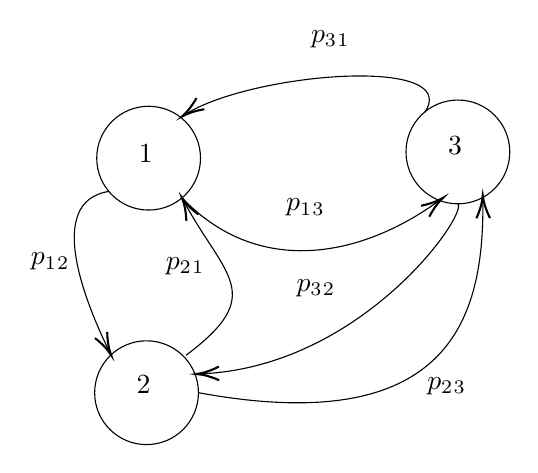
\begin{tikzpicture}[x=0.75pt,y=0.75pt,yscale=-1,xscale=1]
        %uncomment if require: \path (0,300); %set diagram left start at 0, and has height of 300

        %Shape: Circle [id:dp4867332675225031] 
        \draw   (397,111) .. controls (397,97.19) and (408.19,86) .. (422,86) .. controls (435.81,86) and (447,97.19) .. (447,111) .. controls (447,124.81) and (435.81,136) .. (422,136) .. controls (408.19,136) and (397,124.81) .. (397,111) -- cycle ;
        %Shape: Circle [id:dp7153771423061215] 
        \draw   (248,114) .. controls (248,100.19) and (259.19,89) .. (273,89) .. controls (286.81,89) and (298,100.19) .. (298,114) .. controls (298,127.81) and (286.81,139) .. (273,139) .. controls (259.19,139) and (248,127.81) .. (248,114) -- cycle ;
        %Shape: Circle [id:dp10871616919104377] 
        \draw   (247,227) .. controls (247,213.19) and (258.19,202) .. (272,202) .. controls (285.81,202) and (297,213.19) .. (297,227) .. controls (297,240.81) and (285.81,252) .. (272,252) .. controls (258.19,252) and (247,240.81) .. (247,227) -- cycle ;
        %Curve Lines [id:da6335009470514029] 
        \draw    (289,133) .. controls (324.64,170.62) and (374,163.16) .. (413.8,133.89) ;
        \draw [shift={(415,133)}, rotate = 143.13] [color={rgb, 255:red, 0; green, 0; blue, 0 }  ][line width=0.75]    (10.93,-3.29) .. controls (6.95,-1.4) and (3.31,-0.3) .. (0,0) .. controls (3.31,0.3) and (6.95,1.4) .. (10.93,3.29)   ;
        %Curve Lines [id:da03749343666474714] 
        \draw    (406,92) .. controls (413.69,80.66) and (400.89,75.39) .. (380.93,74.53) .. controls (352.34,73.29) and (309.08,81.1) .. (290.39,93.07) ;
        \draw [shift={(289,94)}, rotate = 325.01] [color={rgb, 255:red, 0; green, 0; blue, 0 }  ][line width=0.75]    (10.93,-3.29) .. controls (6.95,-1.4) and (3.31,-0.3) .. (0,0) .. controls (3.31,0.3) and (6.95,1.4) .. (10.93,3.29)   ;
        %Curve Lines [id:da7738798449740533] 
        \draw    (291,209) .. controls (330.4,179.45) and (309.65,171.24) .. (289.9,134.69) ;
        \draw [shift={(289,133)}, rotate = 62.24] [color={rgb, 255:red, 0; green, 0; blue, 0 }  ][line width=0.75]    (10.93,-3.29) .. controls (6.95,-1.4) and (3.31,-0.3) .. (0,0) .. controls (3.31,0.3) and (6.95,1.4) .. (10.93,3.29)   ;
        %Curve Lines [id:da012364105921957802] 
        \draw    (254,130) .. controls (221.83,134.88) and (243.84,186.33) .. (254.22,207.44) ;
        \draw [shift={(255,209)}, rotate = 243.43] [color={rgb, 255:red, 0; green, 0; blue, 0 }  ][line width=0.75]    (10.93,-3.29) .. controls (6.95,-1.4) and (3.31,-0.3) .. (0,0) .. controls (3.31,0.3) and (6.95,1.4) .. (10.93,3.29)   ;
        %Curve Lines [id:da12833590321119237] 
        \draw    (297,227) .. controls (420.75,249.77) and (434.73,188.25) .. (434.03,133.65) ;
        \draw [shift={(434,132)}, rotate = 88.96] [color={rgb, 255:red, 0; green, 0; blue, 0 }  ][line width=0.75]    (10.93,-3.29) .. controls (6.95,-1.4) and (3.31,-0.3) .. (0,0) .. controls (3.31,0.3) and (6.95,1.4) .. (10.93,3.29)   ;
        %Curve Lines [id:da9638645500284003] 
        \draw    (422,136) .. controls (426.98,140.98) and (375.52,215.25) .. (297.18,217.96) ;
        \draw [shift={(296,218)}, rotate = 358.55] [color={rgb, 255:red, 0; green, 0; blue, 0 }  ][line width=0.75]    (10.93,-3.29) .. controls (6.95,-1.4) and (3.31,-0.3) .. (0,0) .. controls (3.31,0.3) and (6.95,1.4) .. (10.93,3.29)   ;

        % Text Node
        \draw (267,106.4) node [anchor=north west][inner sep=0.75pt]    {$1$};
        % Text Node
        \draw (266,217.4) node [anchor=north west][inner sep=0.75pt]    {$2$};
        % Text Node
        \draw (416,102.4) node [anchor=north west][inner sep=0.75pt]    {$3$};
        % Text Node
        \draw (215,158.4) node [anchor=north west][inner sep=0.75pt]    {$p_{1}{}_{2}$};
        % Text Node
        \draw (280,160.4) node [anchor=north west][inner sep=0.75pt]    {$p_{2}{}_{1}$};
        % Text Node
        \draw (338,132.4) node [anchor=north west][inner sep=0.75pt]    {$p_{1}{}_{3}$};
        % Text Node
        \draw (350,51.4) node [anchor=north west][inner sep=0.75pt]    {$p_{3}{}_{1}$};
        % Text Node
        \draw (406,218.4) node [anchor=north west][inner sep=0.75pt]    {$p_{2}{}_{3}$};
        % Text Node
        \draw (343,171.4) node [anchor=north west][inner sep=0.75pt]    {$p_{3}{}_{2}$};


    \end{tikzpicture}
\end{center}

\begin{example}
    Consideriamo un sistema di due bit collegati ai lanci di una moneta con la seguente legge:
    se la moneta da testa viene flippato il primo bit, altrimenti viene flippato il secondo. Assumiamo
    inoltre che la moneta non sia truccata e quindi
    $$\mathbb{P}(T)= \mathbb{P}(C) = \frac{1}{2}.$$
    La matrice di transizione che ne deriva è
    $$P = \begin{matrix}
            [00] \\
            [01] \\
            [10] \\
            [11]
        \end{matrix}\overset{\text{[00] [01] [10] [11]}}
        {\begin{pmatrix}
                0           & \frac{1}{2} & \frac{1}{2} & 0           \\
                \frac{1}{2} & 0           & 0           & \frac{1}{2} \\
                \frac{1}{2} & 0           & 0           & \frac{1}{2} \\
                0           & \frac{1}{2} & \frac{1}{2} & 0
            \end{pmatrix}}$$
    $\boldsymbol{q}=(q_1,q_2,q_3,q_4)$ è il vettore di probabilità iniziale, dove $q_1$ indica la probabilità di iniziare da $[00]$.
    Calcoliamo la probabilità che da un $[ij]$ stato di partenza ottenga tutte le altre configurazioni al primo passo:
    \begin{itemize}
        \item [-]$\mathbb{P}(X_1=[00]) = \frac{1}{2}(q_2+q_3)$
        \item [-]$\mathbb{P}(X_1=[01]) = \frac{1}{2}(q_1+q_4)$
        \item [-]$\mathbb{P}(X_1=[10]) = \frac{1}{2}(q_1+q_4)$
        \item [-]$\mathbb{P}(X_1=[11]) = \frac{1}{2}(q_2+q_3)$
    \end{itemize}
    Quindi l'analisi del primo passo del processo sarà:
    $$\text{passo 1} \to(\frac{1}{2}(q_2+q_3),\frac{1}{2}(q_1+q_4),\frac{1}{2}(q_1+q_4),\frac{1}{2}(q_2+q_3))$$
    Il calcolo svolto per ottenere il vettore probabilità del primo passo non è altro che il prodotto vettore per matrice
    $\boldsymbol{q} \cdot P$. Da questa osservazione segue che possiamo ridurre la computazione di ogni passo ad un prodotto del vettore
    risultante dal passo precedente per la matrice di transizione, che rimane invariata.
    $$\boldsymbol{q_1} = \boldsymbol{q}\cdot P$$
    $$\boldsymbol{q_2} =\boldsymbol{q_1}\cdot P= \boldsymbol{q}\cdot P^2$$
    $$\vdots$$
    $$\boldsymbol{q_n} = \boldsymbol{q_{n-1}}\cdot P = \boldsymbol{q}\cdot P^n$$
\end{example}
\begin{remark}
    Se la matrice $P$ è diagonalizzabile, ovvero è simile ad una matrice diagonale, allora $P$ può essere
    scritta come $P=U^{-1}DU$, dove $D$ è la matrice diagonale. Grazie alla diagonalizzazione abbiamo un modo
    più semplice per calcolare le potenze di matrici, infatti
    $$P^n = (U^{-1}DU)(U^{-1}DU)\dotsb (U^{-1}DU) = U^{-1}D^nU$$
    ma la potenza della matrice diagonale è $D^n = (a_{ij}^n)$.
\end{remark}
\begin{definition}
    Sia $P$ una matrice quadrata, $p_{ij}$ gli elementi della matrice dove $p_{ij}\in[0,1]$ e $\sum_j p_{ij} = 1$,
    allora $P$ è detta \textit{matrice stocastica}.
\end{definition}
\begin{example}
    Consideriamo il processo dell'esempio precedente, consideriamo solo i passi pari del processo, per analizzare i passi del processo dobbiamo calcolare
    la probabilità di andare da $i\to j$ in due passi.
    $$\sum_k p_{ik}p_{kj}\rightarrow\text{probabilità di andare da i a j in due passi}$$
    La nuova matrice di transizione $P' = (\sum_k p_{ik}p_{kj})$  è stocastica.
\end{example}
\begin{example}
    Consideriamo ora due $MC$ sullo stesso $\mathcal{S}$:
    $$ P\to \text{passi pari}$$
    $$ Q\to \text{passi dispari}$$
    Possiamo rappresentare il processo come un alternanza delle matrici stocastiche $P$ e $Q$
    $$\boldsymbol{q}PQPQP\dots$$
    Allo stesso modo possiamo considerare  $PQ=R$ con $r_{ij} = \sum_k p_{ik}q_{kj}$, ottenendo comunque una matrice stocastica $R$,
    quindi il prodotto di matrici stocastiche è una matrice stocastica.
\end{example}
\begin{remark}
    Chiamiamo $p^{(n)}_{ij}$ la probabilità di transizione per andare dallo stato $i$ allo stato $j$ in $n$ passi,
    nell'esempio precedente $\mathbf{(1.4)}$ abbiamo calcolato la probabilità $i\to j$ saltando di due passi
    $$ p^{(2)}_{ij} = \sum_{k\in\mathcal{S}} p_{ik}p_{kj}.$$
    Nel caso generale abbiamo che
    $$p^{(m+n)}_{ij} = \sum_{k\in\mathcal{S}} p^{(m)}_{ik} p^{(n)}_{kj}$$
    in modo equivalente ma facendo riferimento direttamente alle matrici di transizione:
    $$P^{(m+n)} = P^{(m)}\cdot P^{(n)}.$$
    Questa equazione prende il nome di \textit{equazione di Chapman-Kolmogorov}, ricordiamo però che questa è solo una
    versione semplificata delle equazioni perchè stiamo lavorando su $MC$ omogenee.
\end{remark}

\subsection{Stati assorbenti e transienti}
Una serie di risultati interessanti nascono dall'ipotesi di eseguire la $MC$ per molto tempo, e chiedersi quale sia la probabilità che
si finisca in un determinato stato.
\begin{definition}
    Uno stato $i$ è detto assorbente se $p_{ii} = 1$, ovvero una volta entrato in quello stato non potrà più uscirne. Uno stato $j$ è detto \textit{transiente},
    se una volta che il processo lo abbandona, questo non vi ritornerà più.
\end{definition}

\begin{center}


    \tikzset{every picture/.style={line width=0.75pt}}

    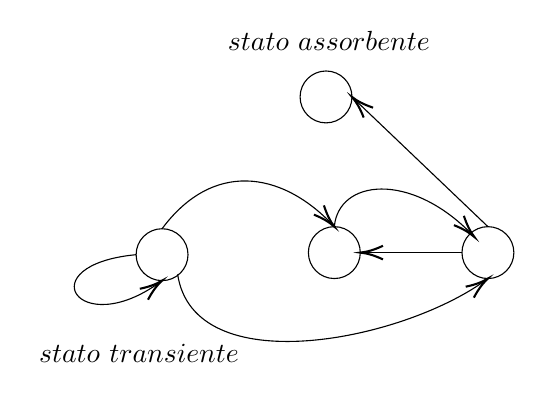
\begin{tikzpicture}[x=0.75pt,y=0.75pt,yscale=-1,xscale=1]

        %Shape: Circle [id:dp59926774136589] 
        \draw   (99,147.5) .. controls (99,140.6) and (104.6,135) .. (111.5,135) .. controls (118.4,135) and (124,140.6) .. (124,147.5) .. controls (124,154.4) and (118.4,160) .. (111.5,160) .. controls (104.6,160) and (99,154.4) .. (99,147.5) -- cycle ;
        %Shape: Circle [id:dp4327123300670961] 
        \draw   (182,146.5) .. controls (182,139.6) and (187.6,134) .. (194.5,134) .. controls (201.4,134) and (207,139.6) .. (207,146.5) .. controls (207,153.4) and (201.4,159) .. (194.5,159) .. controls (187.6,159) and (182,153.4) .. (182,146.5) -- cycle ;
        %Shape: Circle [id:dp4656991214822196] 
        \draw   (256,146.5) .. controls (256,139.6) and (261.6,134) .. (268.5,134) .. controls (275.4,134) and (281,139.6) .. (281,146.5) .. controls (281,153.4) and (275.4,159) .. (268.5,159) .. controls (261.6,159) and (256,153.4) .. (256,146.5) -- cycle ;
        %Straight Lines [id:da5377395097770411] 
        \draw    (256,146.5) -- (209,146.5) ;
        \draw [shift={(207,146.5)}, rotate = 360] [color={rgb, 255:red, 0; green, 0; blue, 0 }  ][line width=0.75]    (10.93,-3.29) .. controls (6.95,-1.4) and (3.31,-0.3) .. (0,0) .. controls (3.31,0.3) and (6.95,1.4) .. (10.93,3.29)   ;
        %Curve Lines [id:da22492685901003262] 
        \draw    (111.5,135) .. controls (135.63,102.49) and (168.5,106.86) .. (193.37,132.8) ;
        \draw [shift={(194.5,134)}, rotate = 227.2] [color={rgb, 255:red, 0; green, 0; blue, 0 }  ][line width=0.75]    (10.93,-3.29) .. controls (6.95,-1.4) and (3.31,-0.3) .. (0,0) .. controls (3.31,0.3) and (6.95,1.4) .. (10.93,3.29)   ;
        %Shape: Circle [id:dp8218498897395967] 
        \draw   (178,71.5) .. controls (178,64.6) and (183.6,59) .. (190.5,59) .. controls (197.4,59) and (203,64.6) .. (203,71.5) .. controls (203,78.4) and (197.4,84) .. (190.5,84) .. controls (183.6,84) and (178,78.4) .. (178,71.5) -- cycle ;
        %Straight Lines [id:da21734777836366703] 
        \draw    (268.5,134) -- (204.45,72.88) ;
        \draw [shift={(203,71.5)}, rotate = 43.66] [color={rgb, 255:red, 0; green, 0; blue, 0 }  ][line width=0.75]    (10.93,-3.29) .. controls (6.95,-1.4) and (3.31,-0.3) .. (0,0) .. controls (3.31,0.3) and (6.95,1.4) .. (10.93,3.29)   ;
        %Curve Lines [id:da5869959620236963] 
        \draw    (99,147.5) .. controls (47.02,152.45) and (71.01,189.25) .. (110.3,160.88) ;
        \draw [shift={(111.5,160)}, rotate = 143.13] [color={rgb, 255:red, 0; green, 0; blue, 0 }  ][line width=0.75]    (10.93,-3.29) .. controls (6.95,-1.4) and (3.31,-0.3) .. (0,0) .. controls (3.31,0.3) and (6.95,1.4) .. (10.93,3.29)   ;
        %Curve Lines [id:da7286336849303717] 
        \draw    (119,157) .. controls (126.92,208.98) and (226.48,189.4) .. (267.28,159.9) ;
        \draw [shift={(268.5,159)}, rotate = 143.13] [color={rgb, 255:red, 0; green, 0; blue, 0 }  ][line width=0.75]    (10.93,-3.29) .. controls (6.95,-1.4) and (3.31,-0.3) .. (0,0) .. controls (3.31,0.3) and (6.95,1.4) .. (10.93,3.29)   ;
        %Curve Lines [id:da2115261987420337] 
        \draw    (194.5,134) .. controls (196.47,111.34) and (230.94,107.12) .. (260.65,137.58) ;
        \draw [shift={(262,139)}, rotate = 226.85] [color={rgb, 255:red, 0; green, 0; blue, 0 }  ][line width=0.75]    (10.93,-3.29) .. controls (6.95,-1.4) and (3.31,-0.3) .. (0,0) .. controls (3.31,0.3) and (6.95,1.4) .. (10.93,3.29)   ;

        % Text Node
        \draw (51,189.4) node [anchor=north west][inner sep=0.75pt]    {$stato\ transiente$};
        % Text Node
        \draw (142,38.4) node [anchor=north west][inner sep=0.75pt]    {$stato\ assorbente$};


    \end{tikzpicture}

\end{center}

Ovviamente essendo una macchina stocastica non può esistere la definizione di stati su cui passeremo un numero finito di volte, se continuiamo il processo per infinito tempo.
Da queste semplici definizioni osserviamo, che se una $MC$ ha uno o più stati assorbenti e  continuiamo il processo per un tempo indeterminato, allora o si finisce in uno degli stati assorbenti,
o ci sono più stati che vengono visitati infinite volte.
\begin{example}
    Consideriamo la $MC$ rappresentata dal grafo non connesso qui sotto:
    \begin{center}


        \tikzset{every picture/.style={line width=0.75pt}}

        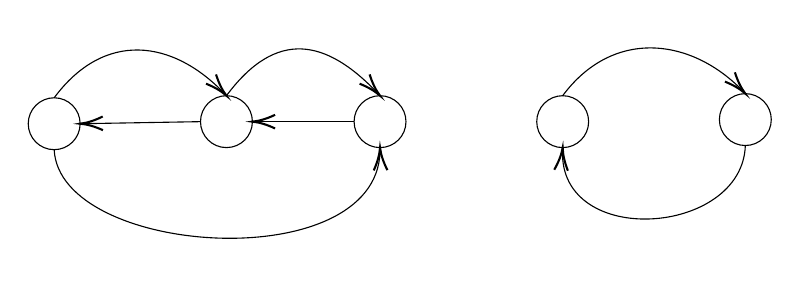
\begin{tikzpicture}[x=0.75pt,y=0.75pt,yscale=-1,xscale=1]

            %Shape: Circle [id:dp59926774136589] 
            \draw   (99,147.5) .. controls (99,140.6) and (104.6,135) .. (111.5,135) .. controls (118.4,135) and (124,140.6) .. (124,147.5) .. controls (124,154.4) and (118.4,160) .. (111.5,160) .. controls (104.6,160) and (99,154.4) .. (99,147.5) -- cycle ;
            %Shape: Circle [id:dp4327123300670961] 
            \draw   (182,146.5) .. controls (182,139.6) and (187.6,134) .. (194.5,134) .. controls (201.4,134) and (207,139.6) .. (207,146.5) .. controls (207,153.4) and (201.4,159) .. (194.5,159) .. controls (187.6,159) and (182,153.4) .. (182,146.5) -- cycle ;
            %Shape: Circle [id:dp4656991214822196] 
            \draw   (256,146.5) .. controls (256,139.6) and (261.6,134) .. (268.5,134) .. controls (275.4,134) and (281,139.6) .. (281,146.5) .. controls (281,153.4) and (275.4,159) .. (268.5,159) .. controls (261.6,159) and (256,153.4) .. (256,146.5) -- cycle ;
            %Shape: Circle [id:dp6233474590560819] 
            \draw   (432,145.5) .. controls (432,138.6) and (437.6,133) .. (444.5,133) .. controls (451.4,133) and (457,138.6) .. (457,145.5) .. controls (457,152.4) and (451.4,158) .. (444.5,158) .. controls (437.6,158) and (432,152.4) .. (432,145.5) -- cycle ;
            %Shape: Circle [id:dp9152667310856856] 
            \draw   (344,146.5) .. controls (344,139.6) and (349.6,134) .. (356.5,134) .. controls (363.4,134) and (369,139.6) .. (369,146.5) .. controls (369,153.4) and (363.4,159) .. (356.5,159) .. controls (349.6,159) and (344,153.4) .. (344,146.5) -- cycle ;
            %Curve Lines [id:da03820678929570742] 
            \draw    (194.5,134) .. controls (218.63,101.49) and (242.77,106.83) .. (267.38,132.8) ;
            \draw [shift={(268.5,134)}, rotate = 227.2] [color={rgb, 255:red, 0; green, 0; blue, 0 }  ][line width=0.75]    (10.93,-3.29) .. controls (6.95,-1.4) and (3.31,-0.3) .. (0,0) .. controls (3.31,0.3) and (6.95,1.4) .. (10.93,3.29)   ;
            %Curve Lines [id:da4658870158499707] 
            \draw    (111.5,160) .. controls (113.98,211.48) and (266.9,221.8) .. (268.5,160.87) ;
            \draw [shift={(268.5,159)}, rotate = 88.64] [color={rgb, 255:red, 0; green, 0; blue, 0 }  ][line width=0.75]    (10.93,-3.29) .. controls (6.95,-1.4) and (3.31,-0.3) .. (0,0) .. controls (3.31,0.3) and (6.95,1.4) .. (10.93,3.29)   ;
            %Straight Lines [id:da5377395097770411] 
            \draw    (256,146.5) -- (209,146.5) ;
            \draw [shift={(207,146.5)}, rotate = 360] [color={rgb, 255:red, 0; green, 0; blue, 0 }  ][line width=0.75]    (10.93,-3.29) .. controls (6.95,-1.4) and (3.31,-0.3) .. (0,0) .. controls (3.31,0.3) and (6.95,1.4) .. (10.93,3.29)   ;
            %Curve Lines [id:da6056089810700547] 
            \draw    (356.5,134) .. controls (380.63,101.49) and (418.35,105.86) .. (443.37,131.8) ;
            \draw [shift={(444.5,133)}, rotate = 227.2] [color={rgb, 255:red, 0; green, 0; blue, 0 }  ][line width=0.75]    (10.93,-3.29) .. controls (6.95,-1.4) and (3.31,-0.3) .. (0,0) .. controls (3.31,0.3) and (6.95,1.4) .. (10.93,3.29)   ;
            %Curve Lines [id:da004797734336944859] 
            \draw    (444.5,158) .. controls (443.02,201.56) and (354.79,207.88) .. (356.42,160.45) ;
            \draw [shift={(356.5,159)}, rotate = 94.09] [color={rgb, 255:red, 0; green, 0; blue, 0 }  ][line width=0.75]    (10.93,-3.29) .. controls (6.95,-1.4) and (3.31,-0.3) .. (0,0) .. controls (3.31,0.3) and (6.95,1.4) .. (10.93,3.29)   ;
            %Curve Lines [id:da22492685901003262] 
            \draw    (111.5,135) .. controls (135.63,102.49) and (168.5,106.86) .. (193.37,132.8) ;
            \draw [shift={(194.5,134)}, rotate = 227.2] [color={rgb, 255:red, 0; green, 0; blue, 0 }  ][line width=0.75]    (10.93,-3.29) .. controls (6.95,-1.4) and (3.31,-0.3) .. (0,0) .. controls (3.31,0.3) and (6.95,1.4) .. (10.93,3.29)   ;
            %Straight Lines [id:da23962912687847093] 
            \draw    (182,146.5) -- (126,147.47) ;
            \draw [shift={(124,147.5)}, rotate = 359.01] [color={rgb, 255:red, 0; green, 0; blue, 0 }  ][line width=0.75]    (10.93,-3.29) .. controls (6.95,-1.4) and (3.31,-0.3) .. (0,0) .. controls (3.31,0.3) and (6.95,1.4) .. (10.93,3.29)   ;




        \end{tikzpicture}

    \end{center}
    formalmente questa è un'unica catena di Markov ma, se ne
    scriviamo la matrice di transizone, sarà una matrice divisa a blocchi.
    \begin{center}


        \tikzset{every picture/.style={line width=0.75pt}} %set default line width to 0.75pt        

        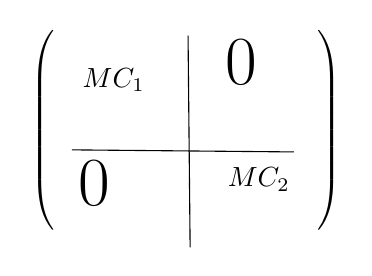
\begin{tikzpicture}[x=0.75pt,y=0.75pt,yscale=-1,xscale=1]

            \draw    (298,108) -- (299,210) ;
            \draw    (242,163) -- (349,164) ;

            % Text Node
            \draw (221,104.4) node [anchor=north west][inner sep=0.75pt]    {$\begin{pmatrix}
                         &        &  &  &        & \\
                         & MC_{1} &  &  &        & \\
                         &        &  &  &        & \\
                         &        &  &  &        & \\
                         &        &  &  & MC_{2} & \\
                         &        &  &  &        &
                    \end{pmatrix}$};
            % Text Node
            \draw (244,167) node [anchor=north west][inner sep=0.75pt]  [font=\Huge] [align=left] {0};
            % Text Node
            \draw (315,109) node [anchor=north west][inner sep=0.75pt]  [font=\Huge] [align=left] {0};


        \end{tikzpicture}

    \end{center}
    Sia $\mathcal{S}=\{1,...,k,k+1,...n\}$
    l'insieme degli stati, dove gli stati da $1$ a $k$ sono rappresentati nel sottografo di sinistra, mentre quelli da $k+1$ ad $n$ a destra.
    Non essendo  i due grafi connessi, una volta che finiremo in uno dei due la probabilità di arrivare ad uno
    qualunque degli stati dell'altro sarà $0$, per questo possiamo rinormalizzare il vettore delle probabilità solo su quelle che riguardano il singolo
    sottografo:
    $$\text{per $1\le i\le k$}\quad \mathbf{q'}=\left(\frac{q_i}{\sum_{i=0}^k q_i}\right) \qquad \text{per $k+1\le i\le n$}\quad \mathbf{q''}=\left(\frac{q_i}{\sum_{i=k+1}^n q_i}\right)$$
\end{example}
Sia $p^{(n)} = \boldsymbol{q}P^n$, supponiamo che $\lim_{n\to\infty}\boldsymbol{q}P^n = \boldsymbol{\pi} $, quindi se lasciamo proseguire il processo
per un tempo illimitato questo si stabilizza e il limite è proprio $\boldsymbol{\pi}$. Inoltre se $\boldsymbol{\pi}$ è il limite otteniamo che
$$\lim_{n\to \infty} \boldsymbol{q}P^n = \lim_{n\to \infty} \boldsymbol{q}P^{n+1} = (\lim_{n\to \infty} \boldsymbol{q}P^n)P = \boldsymbol{\pi} P$$
$$\boldsymbol{\pi}=\boldsymbol{\pi} P.$$
Allora $\boldsymbol{\pi}$ è un autovettore sinistro di $P$, e viene chiamato \textbf{distribuzione stazionaria}. In altre parole,
la distribuzione $\boldsymbol{\pi}$ resta invariata sotto l'evoluzione della catena di Markov. In questo caso, $\boldsymbol{\pi}$ rappresenta una situazione stazionaria in cui, anche se il sistema evolve nel tempo,
la distribuzione complessiva degli stati rimane costante.
\begin{theorem}[Frobenius]
    Una matrice \textit{stocastica} ha sempre un autovalore uguale ad 1.
\end{theorem}
In  generale può succedere che ci siano più autovettori con $\lambda = 1$, chiamiamoli $\boldsymbol{\pi}$ e $\boldsymbol{\pi}'$, che rispettano le seguenti condizioni:
$$ \sum_i \pi_i = 1 \text{ e }\pi_i\ge 0 \text{ per ogni $i$.}$$
Allora possiamo costruire un'altro autovettore che rispetti le precedenti proprietà, quindi sia una distribuzione invariante, facendo una combinazione lineare \textit{convessa} di $\boldsymbol{\pi}$ e $\boldsymbol{\pi}'$:
$$\alpha\boldsymbol{\pi} + (1-\alpha)\boldsymbol{\pi'}\qquad \text{con $\alpha \in [0,1]$.}$$
\subsection{Catene di Markov aperiodiche e irriducibili}
Consideriamo la figura qui sotto con quattro vertici , dove da ogni vertice è
possibile muoversi solo verso quelli adiacenti con una probabilità  $p=\frac{1}{2}$. Chiamiamo inoltre $\boldsymbol{\mu^{(0)}} = (1,0,0,0)$ il vettore che indica
lo stato iniziale (in questo caso scegliamo arbitrariamente di partire da $v_1$).
\begin{center}




    \tikzset{every picture/.style={line width=0.75pt}} %set default line width to 0.75pt        

    \begin{tikzpicture}[x=0.75pt,y=0.75pt,yscale=-1,xscale=1]
        %uncomment if require: \path (0,300); %set diagram left start at 0, and has height of 300

        %Shape: Square [id:dp45511463957766873] 
        \draw   (251,69) -- (379,69) -- (379,197) -- (251,197) -- cycle ;

        % Text Node
        \draw (233,51.4) node [anchor=north west][inner sep=0.75pt]    {$v_{1}$};
        % Text Node
        \draw (379,49.4) node [anchor=north west][inner sep=0.75pt]    {$v_{2}$};
        % Text Node
        \draw (381,200.4) node [anchor=north west][inner sep=0.75pt]    {$v_{3}$};
        % Text Node
        \draw (234,197.4) node [anchor=north west][inner sep=0.75pt]    {$v_{4}$};
        % Text Node
        \draw (302,48.4) node [anchor=north west][inner sep=0.75pt]    {$1/2$};
        % Text Node
        \draw (192,139.4) node [anchor=north west][inner sep=0.75pt]    {$$};


    \end{tikzpicture}


\end{center}
$$ P =\begin{pmatrix}
        0           & \frac{1}{2} & 0           & \frac{1}{2} \\
        \frac{1}{2} & 0           & \frac{1}{2} & 0           \\
        0           & \frac{1}{2} & 0           & \frac{1}{2} \\
        \frac{1}{2} & 0           & \frac{1}{2} & 0           \\
    \end{pmatrix},P^2 =\begin{pmatrix}
        \frac{1}{2} & 0           & \frac{1}{2} & 0           \\
        0           & \frac{1}{2} & 0           & \frac{1}{2} \\
        \frac{1}{2} & 0           & \frac{1}{2} & 0           \\
        0           & \frac{1}{2} & 0           & \frac{1}{2} \\
    \end{pmatrix}, P^3 =\begin{pmatrix}
        0           & \frac{1}{2} & 0           & \frac{1}{2} \\
        \frac{1}{2} & 0           & \frac{1}{2} & 0           \\
        0           & \frac{1}{2} & 0           & \frac{1}{2} \\
        \frac{1}{2} & 0           & \frac{1}{2} & 0           \\
    \end{pmatrix}$$
Se si continuano i calcoli otterremo ciclicamente le stesse matrici, in particolare  per ogni $k\ge 1$
$$P^{2k} = P^2$$
$$P^{2k+1} = P$$
Allo stesso modo vedremo cambiare il vettore delle probabilità $\boldsymbol{\mu^{(n)}}$, che per come è stato scelto sarà sempre uguale alla prima riga di $P^n$.
Catene di Markov con questo tipo di comportamento vengono chiamate \textit{catene periodiche}, in questo caso il \textit{periodo} della catena è uguale a 2.
\begin{definition}
    Il $periodo$ di uno stato $s_i\in\mathcal{S}$ di una catena di Markov è $$d(s_i) = \gcd(n: p_{ii}^{(n)}>0)$$
    lo stato $s_i$ è detto $periodico$ se $d(s_i)>1$.
\end{definition}
Una caratteristica fondamentale delle catene di questo tipo è che possiamo sempre risalire allo stato di partenza, o comunque ad un insieme di stati iniziali compatibili
con il periodo.
Cosa che invece non possiamo dire nel caso in cui  siano \textit{aperiodiche}, infatti le $MC$ per definizione
non hanno memoria.
Nonostante il calcolo delle matrici di transizione sia agevolato dal periodo, le catene periodiche non convergono mai
ad una distribuzione limite: essendo periodica non si fermerà mai in un singolo stato e continuerà ad oscillare
in modo indeterminato tra i $d$ stati  che compongono il periodo. Questa importante proprietà motiva la rimozione della
periodicità da una $MC$.
\begin{remark}
    Affinché una catena di Markov sia periodica è necessario che $p_{ii} = 0$, quindi per rendere la stessa aperiodica sarà sufficiente che
    $$p_{ii} = q$$
    $$p_{ij} = p_{ij}(1-q) \qquad \text{con $q\in(0,1]$}$$
\end{remark}
Possiamo applicare $(1.10)$ all'esempio precedente aggiungendo ad ogni vertice la probabilità $q=1/2$, di restare in quello stesso stato , e $p' = pq$ per andare in uno dei vertici adiacenti.
Quindi la probabilità di rimanere nello stesso stato in cui il processo si trovava al passo precedente "distrugge" la periodicità della catena.
\begin{definition}
    Una catena di Markov è detta \textit{aperiodica} se $d(s_i)\le 1$ per ogni stato $s_i\in\mathcal{S}$, ovvero se nessuno stato è periodico.
\end{definition}
\begin{definition}
    Diciamo che $i$ $comunica$ con $j$ ($i\to j$) se esiste $n\in \mathbb{Z}^+$ tale che $p^{(n)}_{ij}>0$, quindi se esiste un certo numero di passi
    per andare da $i$ a $j$. Nel caso in cui volessimo dare una condizione per le catene non omogenee diremo che $i$ comunica con $j$ se $$\mathbb{P}(X_{m+n}=s_j|X_{m} =s_i)>0$$
\end{definition}
\begin{definition}
    $i$ e $j$ sono $comunicanti$ se $i\to j$ e $j\to i$ ($i\longleftrightarrow j$).
\end{definition}
\begin{definition}
    Una catena di Markov è \textit{irriducibile} se $i\longleftrightarrow  j$ per ogni $i,j\in \mathcal{S}$, altrimenti è detta \textit{riducibile}.
\end{definition}
La catena dell'esempio $\mathbf{(1.8)}$, rappresentata come un grafo non connesso, è una catena di Markov \textit{riducibile}. Ogni catena di Markov $riducibile$
può essere rappresentata con una matrice di transizione divisa a blocchi. Lo studio di una $MC$ divisa in blocchi è ridotto allo studio delle $MC$ $irriducibili$ che la compongono.\\
\begin{theorem}
    Supponiamo di avere una catena di Markov ($X_0,X_1,\dots$)  $aperiodica$ con spazio degli stati $\mathcal{S} = \{s_1,\dots s_k\}$ e matrice di transizione $P$. Allora esiste $N<\infty$ tale che
    $$(P^n)_{ii}>0\quad $$
\end{theorem}
Per provare il seguente risultato abbiamo bisogno del seguente $lemma$ relativo alla \textit{teoria dei numeri}.
\begin{lemma}
    Sia $A=\{a_1,a_2,\dots\}$ con $a_i\in\mathbb{N}$ con le seguenti proprietà:
    \begin{itemize}
        \item [-] non è reticolare ($\gcd(a_1,a_2,\dots) = 1$)
        \item [-] chiuso rispetto all'addizione.
    \end{itemize}
    Allora esiste $N<\infty$ tale che $n\in A$  per ogni  $n\ge N$.
\end{lemma}
\begin{proof}[\textbf{Dimostrazione} (Teorema 1.16)] Consideriamo $s_i\in\mathcal{S}$ e associato ad esso l'insieme $$A_i =\{n\ge 1|\text{ } p^{(n)}_{ii}>0\}$$
    rappresentante la collezione di \textit{tempi di ritorno} di uno stato in se stesso. Abbiamo assunto che la $MC$ sia aperiodica, da questo segue che $A_i$ sia un
    insieme \textit{non reticolare}. Per servirci del lemma precedente dobbiamo provare che $A_i$ sia anche chiuso rispetto alla somma, quindi che presi $a,a'\in A_i$,
    allora $a+a'\in A_i$. Dato che $a,a' \in A_i$ abbiamo che: $$\mathbb{P}(X_a =s_i | X_0 =s_i)>0$$
    $$\mathbb{P}(X_{a'}= s_i|X_0 = s_i) = \mathbb{P}(X_{a'+a}= s_i| X_a = s_i)>0$$
    Dalle precedenti ricaviamo
    \begin{align*}
        \mathbb{P}(X_{a+a'} = s_i| X_0 = s_i) \ge \mathbb{P}(X_{a+a'}= s_i, X_a =s_i| X_0 = s_i) \\
        =\mathbb{P}(X_{a} = s_i|X_0 = s_i) \mathbb{P}(X_{a+a'} = s_i | X_a = s_i) > 0
    \end{align*}
    quindi $a+a'\in A_i$. Segue che esiste $N_i$ tale che ogni $a>N_i$ appartiene ad $A_i$, in altre parole la probabilità di ritorno da $i\to i$, dopo $N_i$ passi, è sempre positiva. Segue
    che $N = \max_{i\in |\mathcal{S}|}\{N_i\}$ è il limite di passi oltre il quale $(P^n)_{ii} > 0 $ per ogni $i$.
\end{proof}
Combinando \textit{aperiodicità} e \textit{irriducibilità} otteniamo il seguente risultato che ci tornerà utile nella dimostrazione del \textit{teorema di convergenza delle catene di Markov}.
\begin{corollary}
    Sia ($X_0,X_1\dots$) una catena di Markov $irriducibile$ e $aperiodica$ con spazio degli stati $\mathcal{S} =\{s_1,s_2\dots s_l\}$ e matrice di
    transizione $P$. Allora esiste $M<\infty$ tale che $(P^n)_{ij}>0$ per ogni $i,j\in\{1,\dots k\}$ ed ogni $n\ge M$.
\end{corollary}
\begin{example}[Passeggiata su un toro discreto]
    Siano $a$ e $b$ due interi positivi, e consideriamo la catena di Markov con spazio degli stati
    $$\mathbb{T}^2(a,b):=\{(x,y) | x\in \{0,1\dots a-1\}, y \in \{0,1,\dots b-1\}\}$$
    e il seguente meccanismo di transizione: se la catena è nello stato $(x,y)$ al tempo $n$, allora al tempo $n+1$ sarà nello stato $((x+1)\mod a,y)$ o $(x,(y+1) \mod b)$,
    ciascuno con probabilità $\frac{1}{2}$. Chiaramente è una catena di Markov $irriducibile$, in quanto dati due stati $(x',y')$ e  $(x,y)$,
    allora possiamo spostarci di una serie di passi  in modo che $x+p \equiv x' \mod a$ e $y+q \equiv y'\mod b$, in entrambi i casi con probabilità positiva pari a
    $$\mathbb{P}(X_{p+q} = (x',y')| X_0 = (x,y)) = \left(\frac{1}{2}\right)^{p+q} $$
    ne segue che ogni coppia di stati è comunicante, quindi la catena è $irriducibile$. Mostriamo ora che la catena è $aperiodica$ se e solo se  $\gcd(a,b) = 1$. Supponiamo
    di trovarci in un punto generico $(z,w)$ di $\mathbb{T}^2(a,b)$, per tornare in $(z,w)$ allora possiamo scegliere di fare $a$ passi orizzontali o $b$ passi verticali, altrimenti una
    combinazione dei due, in ogni caso sarà un numero $ka+tb$ di passi, quindi $d(z,w) = \gcd(a,b,2a,2b,2a+b,\dots) = 1 \iff  \gcd(a,b) = 1$.
\end{example}
\subsection{Simulazione di una catena di Markov}
Consideriamo una successione di variabili aleatorie $X_0,X_1\dots$ rappresentanti la traiettoria di una catena di Markov omogenea, con $\mathbb{P}(X_n = i| X_{n-1}= j) = p_{ij}$.
Per simulare una catena di Markov abbiamo bisogno di una successione di variabili aleatorie
$$U_0,U_1\dots\qquad  \text{$U_i$ uniformi su $[0,1]$ e sono indipendenti}$$
quindi $\mathbb{P}(U_i\le x) = \int_0^x dx$. Lo spazio degli stati deve essere finito e periodico,
il periodo deve essere maggiore del numero di $v.a.$ utilizzate. In questo modo si evita la ripetizione di pattern quando
si ripassa su uno stesso stato. Oltre alla successione $\{U_i\}$ dobbiamo definire due funzioni, una per l'inizializzazione
ed una per l'aggiornamento:
\begin{itemize}
    \item[-] \textit{inizializzazione} : $\psi : I\to \mathcal{S}$, da $[0,1]$ scelgo uno stato da cui iniziare.
          Per ogni $s\in\mathcal{S}$, la lunghezza di un intervallo in cui $\psi(x)=s$ deve essere $\mu^{(0)}(s) =\mathbb{P}(X_0 = s) $.
          Definiamo $\mu^{(0)}(s)$ come la misura dell'intervallo che rappresenta lo stato $s$ al passo $0$, ovvero
          $$ \mu^{(0)} = \mathbb{P}(X_0 = s) = \mathbb{P}(\psi(U_0)=s) = \int_0^1 \chi_{\{\psi(x)=s\}} dx$$
          dove $\chi_{\{\psi(x) = s\}}$ è la funzione caratteristica sull'insieme dei punti  $x\in [0,1]$, tali che $\psi(x) = s$
          $$\chi_{\{\psi(x) = s\}} =\left\{ \begin{array}{cl} 1 \quad \psi(x) = s\\ 0 \quad \psi(x) \neq s\end{array} \right.$$
          Diamo ora una semplice costruzione della funzione $\psi$ costante a tratti:
          $$\psi(x)= \begin{cases}

                  s_1 \quad \text{per $x\in [0,\mu^{(0)}(s_1))$}                             \\
                  s_2 \quad \text{per $x\in [\mu^{(0)}(s_1),\mu^{(0)}(s_1)+\mu^{(0)}(s_2))$} \\
                  \vdots                                                                     \\
                  s_i \quad \text{per $x \in [\sum_{j=1}^{i-1}\mu^{(0)}(s_j),\sum_{j=1}^i\mu^{(0)}(s_j))$}
                  \vdots                                                                     \\
                  s_k \quad \text{per $x\in[\sum_{j=1}^{k-1}\mu^{(0)}(s_j),1]$}
              \end{cases}$$
    \item[-]\textit{update}: $\phi : [0,1]\times\mathcal{S}\to \mathcal{S} $, $\phi$ prende in input sia il numero casuale della $v.a$ $U_i$ (con $i>0$), sia  lo stato attuale.
          La funzione definisce in quale stato il processo arriverà, sulla base dello stato da cui parte e il numero tra $0$ e $1$ appena generato. Possiamo costruire $\phi$ in modo simile
          a quello usato con $\psi$, in questo caso però $\phi$ rappresenterà la probabilità di transizione.
\end{itemize}
Quindi la simulazione della catena non sarà altro che una successione di variabili aleatorie uniformi a cui applichiamo inizialmente $\psi$, successivamente aggiorniamo
il suo stato con $\phi$:
$$X_0 = \psi(U_0),\quad X_1 = \phi(U_1,s_q),\quad  \cdots X_n = \phi(U_n,s_k)$$
\begin{remark}
    Nel caso in cui si volesse simulare una $MC$ non omogenea  dovremmo modificare la funzione di update ad ogni passo, e quindi dovremmo avere un $\phi_i$ per ogni $i$-esimo passo, oppure  una funzione in tre variabili :
    $$\widehat{\phi}:[0,1]\times\mathcal{S}\times \mathbb{Z}^+\to \mathcal{S}$$
    dove l'intero indica il tempo (discreto) in cui il processo si trova.
\end{remark}
\subsection{Distribuzione stazionaria}
Anche se già incontrata in precedenza, diamo ora  una definizione formale di distribuzione stazionaria per una catena di Markov.
\begin{definition}
    Sia ($X_0,X_1,\dots$) una catena di Markov con spazio degli stati $\{s_1,s_2\dots s_k\}$ e matrice di transizione $P$. Il vettore
    $\boldsymbol{\pi} = (\pi_1,\pi_2\dots\pi_k)$ è detta distribuzione stazionaria se soddisfa le seguenti condizioni:
    \begin{itemize}
        \item [\textit{(i)}] $\pi_i\ge 0$ per $i = 1,\dots k$ e $\sum_{i=1}^k \pi_k = 1$ e
        \item [\textit{(ii)}]$\boldsymbol{\pi}P = \boldsymbol{\pi}$, ovvero $\sum_{i=1}^k \pi_i P_{ij} = \pi_j$ per $j =1,\dots k$.
    \end{itemize}
\end{definition}
Consideriamo uno stato arbitrario di partenza $X_0= i$ e definiamo $$T_{ij} :=\min\{n\ge 1| X_n = j\},$$ come il \textit{tempo aleatorio} per andare dallo stato
$i$ allo stato $j$, sia invece $\tau_{ij} := \mathbb{E}(T_{ij})$. Nel caso in cui $i=j$ chiameremo $T_i$  come il $tempo$ $di$ $ritorno$ e, se $s_j$ non fosse raggiungibile da $s_i$, $T_{ij} = \infty$.
\begin{proposition}
    Sia $(X_0,X_1,\dots)$ un catena $aperiodica$ ed $irriducibile$, allora $$\mathbb{P}(T_{ij}<\infty) =1 \text{ e } \tau_{ij}<\infty\text { per ogni $i,j$}.$$
\end{proposition}
\begin{proof}[\textbf{Dimostrazione}]
    Come dimostrato in precedenza, esiste sempre un certo intero positivo $M$ tale che $p_{ij}^{(M)}>0$ per ogni $i,j$. Prendiamo la probabilità di transizione minima $\alpha = \min_{i,j} (p_{ij}^{(M)})$ in $P^{(M)}$, con la quale otteniamo
    la seguente disuguaglianza:
    $$\mathbb{P}(T_{ij}>M)\le \mathbb{P}(X_M \neq j)\le  1-\alpha$$
    quindi
    \begin{align*}
        \mathbb{P}(T_{ij}>2M) = \mathbb{P}(T_{ij}>M)\mathbb{P}(T_{ij}>2M | T_{ij}>M) \\
        \le\mathbb{P}(T_{ij}>M)\mathbb{P}(X_{2M}\neq j| T_{ij}>M)\le (1-\alpha)^2
    \end{align*}
    iterando questo processo $\ell$ volte avremo
    $$\mathbb{P}(T_{ij}>\ell M)\le (1-\alpha)^{\ell}.$$
    Quando $\ell$ tende ad infinito $$\mathbb{P}(T_{ij}>\infty)  = 0$$
    passando al complemento otteniamo il primo risultato. Per il secondo punto sviluppiamo la sommatoria del
    valore atteso:
    \begin{align*}
        \mathbb{E}(T_{ij}) & = \sum_{n=1}^{\infty}\mathbb{P}(T_{ij}\ge n) = \sum_{n=0}^{\infty}\mathbb{P}(T_{ij}> n)                                                                          \\
                           & =\sum_{\ell = 0}^{\infty}\sum_{n = \ell M}^{(\ell+1)M-1}\mathbb{P}(T_{ij}>n)  \le\sum_{\ell = 0}^{\infty}\sum_{n =\ell M}^{(\ell+1)M-1}\mathbb{P}(T_{ij}>\ell M) \\
                           & = M\sum_{\ell = 0}^{\infty} \mathbb{P}(T_{ij}>\ell M) \le M\sum^{\infty}_{\ell = 0} (1-\alpha)^{\ell} = M\frac{1}{1-(1-\alpha)} = \frac{M}{\alpha}<\infty
    \end{align*}
\end{proof}
\begin{theorem}
    Una catena $irriducibile$ e $aperiodica$ ha almeno una distribuzione stazionaria.
\end{theorem}
\begin{proof}[\textbf{Dimostrazione}]
    Consideriamo la catena di Markov ($X_0,X_1,\dots)$, $irriducibile$ e $aperiodica$, con stati $\mathcal{S} = \{s_1,s_2\dots s_k\}$ e matrice di transizione
    $P$. Supponiamo che la catena inizi nello stato $s_1$, quindi $X_0 = s_1$ e definiamo
    $$\rho_i = \sum_{n = 0}^{\infty}  \mathbb{P}(X_n = s_i \cap \, T_{11}>n)$$
    come il numero medio di visite che faccio allo stato $i$, partendo da $s_1$ e tornandoci in un tempo maggiore di $n$. Dato che $\mathbb{E}(T_{11}) = \tau_{11}$, e $rho_i<\tau_{11}$ per ogni $i$, otteniamo
    che $\rho_i$ è finito. Possiamo allora costruire un vettore candidato ad essere la nostra distribuzione stazionaria:
    $$\pi =(\pi_1,\pi_2,\dots,\pi_k) =  \left(\frac{\rho_1}{\tau_{11}},\frac{\rho_2}{\tau_{11}},\dots,\frac{\rho_k}{\tau_{11}}\right)$$
    Scelto $\pi$ come sopra, non ci resta che dimostrare le due proprietà di una distribuzione stazionaria.\\
    Per prima cosa dimostriamo che vale $\pi_j = \sum_i^k \pi_i Pij$ per $j\neq 1$, caso che tratteremo separatamente:
    \begin{align*}
        \pi_j = \frac{\rho_j}{\tau_{11}} = & \frac{1}{\tau_{11}}\sum_{n = 0}^{\infty}\mathbb{P}(X_n = s_j \cap T_{11}>n)                                                                      \\
        =                                  & \frac{1}{\tau_{11}}\sum_{n = 1}^{\infty}\mathbb{P}(X_n = s_j \cap T_{11}>n)                                                                      \\
        =                                  & \frac{1}{\tau_{11}}\sum_{n = 1}^{\infty}\mathbb{P}(X_n = s_j \cap T_{11}>n-1)                                                                    \\
        =                                  & \frac{1}{\tau_{11}}\sum_{n = 1}^{\infty}\sum_{i=1}^k\mathbb{P}(X_n = s_j,\, X_{n-1} = s_i,\,T_{11}>n-1)                                          \\
        =                                  & \frac{1}{\tau_{11}}\sum_{n = 1}^{\infty}\sum_{i=1}^k\mathbb{P}( X_{n-1} = s_i,\,T_{11}>n-1)\mathbb{P}(X_n = s_j|X_{n-1} = s_i)                   \\
        =                                  & \frac{1}{\tau_{11}}\sum_{i=1}^kP_{ij}\sum_{n = 1}^{\infty}\mathbb{P}( X_{n-1} = s_i,\,T_{11}>n-1) =  \frac{1}{\tau_{11}}\sum_{i=1}^k\rho_iP_{ij} \\
        =                                  & \sum_{i=1}^k\pi_iP_{ij}
    \end{align*}
    Verifichiamo ora la condizione precedente anche per il caso in cui $j=1$, chiaramente $\rho_1 = 1$ per definizione, da questo otteniamo
    \begin{align*}
        \pi_1 = \frac{\rho_1}{\tau_{11}} & = \frac{1}{\tau_{11}} \mathbb{P}(T_{11}<\infty) = \frac{1}{\tau_{11}} \sum_{n = 1}^{\infty}\mathbb{P}(T_{11} = n)                                                                   \\
                                         & =\frac{1}{\tau_{11}} \sum_{n= 1}^{\infty}\sum_{i = 1}^{k}\mathbb{P}(X_{n-1} = s_i,T_{11} = n)                                                                                       \\
                                         & =\frac{1}{\tau_{11}} \sum_{n= 1}^{\infty}\sum_{i = 1}^{k}\mathbb{P}(X_{n-1} = s_i,T_{11} > n-1)\mathbb{P}(X_n=s_1|X_{n-1}= s_i)                                                     \\
                                         & =\frac{1}{\tau_{11}}  \sum_{i = 1}^{k}P_{i1}\sum_{n= 1}^{\infty}\mathbb{P}(X_{n-1} = s_i,T_{11} > n-1) \quad (\text{scrivo }m = n-1)                                                \\
                                         & = \frac{1}{\tau_{11}} \sum_{i = 1}^{k}P_{i1}\sum_{m= 0}^{\infty}\mathbb{P}(X_{m} = s_i,T_{11} > m) =\frac{1}{\tau_{11}}  \sum_{i = 1}^k \rho_i P_{i1} = \sum_{i = 1}^k \pi_i P_{i1}
    \end{align*}
    Ci rimane ora da verificare che $\sum_{i}\pi_i = 1$, ma questo segue dalla seguente osservazione:
    \begin{align*}
        \tau_{11} = \mathbb{E}(T_{11}) & = \sum_{n=0}^{\infty} \mathbb{P}(T_{11}<n)                                            \\
                                       & =\sum_{n=0}^{\infty}\sum_{i=1}^k \mathbb{P}(X_{n} = s_i,T_{11}<n)                     \\
                                       & = \sum_{i=1}^k\sum_{n=0}^{\infty}\mathbb{P}(X_{n} = s_i,T_{11}<n)=\sum_{i=1}^k \rho_i \\
    \end{align*}
    e quindi $\sum_i \pi_i = \sum_{i=1}^k\tau_{11}^{-1} \rho_i = 1$.
\end{proof}
Ora che sappiamo dell'esistenza della distirbuzione, possiamo studiare il comportamento asintotico di una distirbuzione $\mu^{(n)}$, con distribuzione iniziale arbitraria $\mu^{(0)}$. Per parlare di convergenza, dobbiamo
obbligatoriamente introdurre una definizione di distanza.
\begin{definition}
    Se $\nu' = (\nu_1',\nu_2',\dots,\nu_k')$ e $\nu'' =(\nu_1',\nu_2',\dots,\nu_k'')$ sono distribuzioni su $\mathcal{S} = \{s_1,s_2\dots s_k\}$, definiamo la \textbf{\textit{distanza di variazione totale}} tra $\nu'$ e $\nu''$:
    $$d_{TV}(\nu',\nu'') = \frac{1}{2}\sum_{i=1}^k|\nu_i'-\nu_i''|.$$
    Se $\nu^{(1)},\nu^{(2)}\dots$ è una successione di distribuzioni di probabilità su $\mathcal{S}$, allora diremo che  $\nu^{(n)}$
    converge a $\nu$ in $variazione$ $totale$ con $n\to \infty$, scrivendo $\nu^{(n)}\xrightarrow{TV}\nu$, se
    $$\lim_{n\to\infty} d_{TV}(\nu^{(n)},\nu) = 0$$
\end{definition}
\begin{remark}
    Il coefficiente $1\over 2$ in $d_{TV}$ serve a mantenere la distanza tra due distribuzioni, compresa nell'intervallo $[0,1]$, nel caso in cui la distanza $d_{TV}(\nu',\nu'')=0$ allora $\nu' = \nu''$. Se invece è $1$, la loro rispettiva distribuzione sarà concentrata su due
    partizioni disgiunte di $\mathcal{S}$.
\end{remark}
\begin{theorem}[\textbf{Convergenza delle catene di Markov}] Sia $(X_0,X_1,\dots)$ una catena di Markov irriducibile e aperiodica, con spazioe degli stati $\mathcal{S}=\{s_1,\dots,s_k\}$,
    matrice di transizione $P$, e una distribuzione iniziale arbitraria $\mu^{(0)}$. Per ogni distribuzione $\pi$ stazionaria per la matrice $P$, abbiamo
    $$\mu^{(n)}\xrightarrow{TV}\pi$$

\end{theorem}
Per dimostrare il teorema utilizzeremo un metodo probabilistico chiamato \textbf{coupling}, il quale consiste nel realizzare la simulazione di due $MC$, e analizzare quando quest'ultime si incrociano (si trovano nello stesso stato).
\begin{proof}[\textbf{Dimostrazione}]
    Per studiare il comportamento della distribuzione $\mu^{(n)}$, possiamo avanzare l'ipotesi che sia generata da una simulazione
    di catena di Markov, inizializzata e aggiornata come indicato in \textbf{(1.3)}. Quindi la catena $X_0,X_1\dots$ sarà generata da
    \begin{align*}
        X_0 & = \psi_{\mu^{(0)}}(U_0) \\
        X_1 & = \phi(X_0,U_1)         \\
        X_2 & = \phi(X_1,U_2)         \\
            & \vdots
    \end{align*}
    La $\psi_{\mu^{(0)}}$ è  una funzione di inizalizzazione per $\mu^{(0)}$, $\phi$ è la funzione di aggiornamento per la matrice $P$, e come in precedenza
    $U_0,U_1\dots$, sono una sequenza di variabili aleatorie uniformi generate.
    In modo analogo definiamo una seconda catena di Markov, $(X'_0,X_1',\dots)$, con funzione di inizializzazione $\psi_{\pi}$ per la distribuzione $\pi$ e $(U_0',U_1'\dots)$ un'altra sequenza di variabili aleatorie uniformi.
    Dato che $\pi$ è una distribuzione stazionaria, avremo che $X_n'$ avrà distribuzione $\pi$ per ogni $n$. Otteniamo quindi:
    \begin{align*}
        X_0' & = \psi_{\pi}(U_0') \\
        X_1' & = \phi(X_0',U_1')  \\
        X_2' & = \phi(X_1',U_2')  \\
             & \vdots
    \end{align*}
    Ovviamente le due successioni ($X_0,X_1\dots)$ e $(X_0',X_1',\dots)$ sono indipendenti, come le loro rispettive successioni di variabili aleatorie uniformi. Vogliamo dimostrare che per un certo $n$ le due catene si incontrano con probabilità $1$, ovvero $\mathbb{P}(X_n = X_n') = 1$.
    Definiamo $T$ come il primo tempo di incontro tra le due catene, ovvero $T  =\min\{n:X_n = X_n'\}$. Come dimostrato nel corollario \textbf{(1.18)}, dato che la catena è ergodica, possiamo trovare un intero $M<\infty$, tale che
    $$P_{ij}^{(M)}>0\qquad \text{per ogni }i,j\in\{1,\dots k\}.$$
    Sia
    $$\alpha = \min\{P_{ij}^{(M)}| i\in\{1,\dots k\},$$
    otteniamo che
    \begin{align*}
        \mathbb{P}(T\le M) & \ge \mathbb{P}(X_M = X_M')  \ge\mathbb{P}(X_M = s_1, X_M' = s_1)                                                                                                \\
                           & \overset{indip.}{=} \mathbb{P}(X_M = s_1) \mathbb{P}(X_M'=s_1)                                                                                                  \\
                           & =\left(\sum_{i=1}^k \mathbb{P}(X_0 = s_i, X_M = s_1)\right)\left(\sum_{i=1}^k \mathbb{P}(X_0' = s_i, X_M' = s_1)\right)                                         \\
                           & =\left(\sum_{i=1}^k \mathbb{P}(X_0 = s_i)\mathbb{P}(X_M =s_1|X_0 = s_i)\right)\left(\sum_{i=1}^k \mathbb{P}(X_0' = s_i)\mathbb{P}(X_M' = s_1| X_0' =s_i)\right) \\
                           & \ge \left(\alpha\sum_{i= 1}^k\mathbb{P}(X_0 =s_i)\right)\left(\alpha\sum_{i= 1}^k\mathbb{P}(X_0'=s_i)\right) = \alpha^2
    \end{align*}
    passando al complemento
    $$\mathbb{P}(T>M) \le 1-\alpha^2.$$
    Quindi dato che la probabilità di incontro entro $M$ passi in $s_1$ è maggiore di $\alpha^2$, allora  $\mathbb{P}(X_{2M} \neq X_{2M}' | T>M)\le 1-\alpha^2$.
    Ripetiamo il calcolo ad esempio nel caso in cui il tempo di incontro supera $2M$:
    \begin{align*}
        \mathbb{P}(T>2M) & = \mathbb{P}(T>M)\mathbb{P}(T>2M| T>M)                              \\
                         & \le(1-\alpha^2)\mathbb{P}(T>2M|T>M)                                 \\
                         & \le(1-\alpha^2)\mathbb{P}(X_{2M}\neq X_{2M}'|T>M)\le (1-\alpha^2)^2 \\
    \end{align*}
    Reiterando l'argomento per $\ell$ volte otteniamo che:
    $$\mathbb{P}(T>\ell M)\le (1-\alpha^2)^{\ell}$$
    dove se $\ell\to\infty$, allora $(1-\alpha^2)^{\ell}\to 0$, abbiamo quindi dimostrato che la probabilità che  le due catene si incontrino è $1$.
    Definiamo ora una nuova catena di Markov $(X_0'',X_1'',\dots)$ in modo simile alle due precedenti, dichiarando lo stato di partenza $X_0'' = X_0$ e per ogni $n$
    $$X_{n-1}'' =\left\{\begin{array}{cl}
            \phi(X_n'',U_{n+1})\quad se\;X_n'' \neq X_n' \\
            \phi(X_n'',U_{n+1}')\quad se\;X_n'' = X_n'
        \end{array}\right.$$
    in parole, la catena $(X_0'',X_1'',\dots)$ evolve come la catena $(X_0,X_1,\dots)$ fino a che non si incontra con $X_i'$, successivamente
    continua l'evoluzione come $(X_0',X_1'\dots)$. Dato che abbiamo fatto iniziare questa nuova catena da $X_0$, allora la distribuzione di $X_0''$ è $\mu^{(0)}$, quindi per ogni $n$ la distribuzione di $X_n''$ ha distribuzione $\mu^{(n)}$.
    Ora per ogni $i\in\{1,\dots k\}$ otteniamo che
    \begin{align*}
        \mu^{(n)}_i - \pi_i & = \mathbb{P}(X_n'' = s_i) -\mathbb{P}(X_n' = si_i)          \\
                            & \le \mathbb{P}(X_n'' = s_i, X_n' \neq s_i)   \qquad (\star) \\
                            & \le \mathbb{P}(X_n'' \neq X_n')  = \mathbb{P}(T>n)
    \end{align*}
    $(\star)\mathbb{P}(A)-\mathbb{P}(B)\le \mathbb{P}(A\cap B^{\complement}) = \mathbb{P}(A)-\mathbb{P}(A\cap B) \implies \mathbb{P}(B)\ge \mathbb{P}(A\cap B)$\\

    In modo analogo verifichiamo che $\pi_i - \mu^{(n)}_i \le \mathbb{P}(T>n)$, in entrambi i casi se $n\to\infty$, allora $\mathbb{P}(T>n)\to 0$, segue che
    $$\lim_{n\to \infty}|\mu_i^{(n)}-\pi_i| = 0$$
    implicando a sua volta che $\mu^{(n)}\xrightarrow{TV}\pi$ ovvero:
    $$\lim_{n\to\infty}d_{TV}(\mu^{(n)},\pi) = \lim_{n\to\infty}\left(\frac{1}{2}\sum_{i = 1}^k |\mu_i^{(n)}-\pi_i|\right)  = 0$$
\end{proof}
\begin{theorem}[Unicità della distribuzione stazionaria]
    Ogni catena di Markov aperiodica e irriducibile ha esattamente una distribuzione stazionaria.
\end{theorem}
\begin{proof}[Dimostrazione] Segue dal teorema di $convergenza$.

\end{proof}
\end{document}